\chapter{Introduction}

It all started with Darwin's book of The Origins of Species, which he published in 1859. Since then, the field of genomics have been paid a great deal of attention. With the advancing power of computers, the genomic studies had to adapt itself into this new circumstances. The Human Genome Project was started in 1990 with the goal of determining all the bases in human genome. This was not only exciting but also difficult goal to reach since it could take years or decades to sequence the whole genome with the existing technology. As expected, after 13 years of hard work, the results were published in 2003, and it cost \$2.7 billion \cite{costOfHumanGenomeProject}.

The main sequencing method that was used in Human Genome Project was Sanger's chain termination method, or commonly referred to as Sanger sequencing. Sanger sequencing, named after the inventor Frederick Sanger, was good in terms of accuracy, however, it was time-consuming and expensive. In the early 2000s, methods that were better at time and money were finally emerging. Next-generation or high-throughput methods have revolutionized the sequencing business by providing millions of ``reads", short sequences, in a massively parallel fashion at a lower cost. As high-throughput sequencing (HTS) methods have become widespread, an effort to make available as many human genomes as possible was set out. For instance, started in 2008, 1000 Genome Project aimed to sequence approximately 2500 individual coming from different ethnic backgrounds \cite{10002015global}. Several countries, among them are Turkey, have started their own genome projects. In addition to human genome, genomes belonging to other species have also been sequenced \cite{koepfli2015genome}. 

\section{DNA Sequencing}

Before 1950s, the term ``gene" was referred to as the smallest unit of genetic information \cite{crickpapers}. Scientists at that time were identifying the DNA as the carrier of genetic information, however, they knew very little about how a trait passes down to younger generations. In 1953, there was a breakthrough in the field of genomics with the discovery of double helix structure of DNA by James Watson and Francis Crick. Watson and Crick had answered the biggest question till then in genomics that could lead to solving the mystery about genetic heredity. In a series of articles published in several journals, Watson et al., apart from exposing the structure of DNA, have put their findings together with those of other researchers and come up with a mechanism for DNA replication along with three pieces of evidence supporting the complementary model which suggests that adenine has thymine and cytosine has guanine on the opposite strand of DNA, or vice versa \cite{watson1953structure}.

\subsection{Early Sequencing Methods}
The complementary model opens the door of DNA sequencing since it allows the DNA to be reconstructed from one strand. There were some initial thoughts and methods on how to sequence the DNA, however, none of them were practical in terms of speed to sequence the whole genome. Frederick Sanger and Alan Coulson were the first who have developed the ``plus and minus" method, which was soon replaced by chain-termination method, for rapidly determining the order of smallest genetic units in DNA\cite{sanger1975rapid}. In an article published in 1970, Sanger et al. have set the gold standard in sequencing. They used DNA polymerase, an enzyme that is essential for DNA replication, to generate copy DNA sequences from the template DNA strand, all of which should start in the same exact position and end in normally one base larger (and heavier) than the previous. Sanger was able to stop the polymerase by removing an oxygen from the nucleotide at which he wants to stop. Sanger made these DNA sequences move at a speed such that the fewer nucleotides they have, the faster they are. Nucleotides will emit a light in different wavelengths, hence, from a fixed point of view, a light sensor will be able to detect the sequence of nucleotides. 

\subsubsection{Human Genome Project}
As the technology in DNA sequencing advances, it has become a must to sequence the whole human genome. After two years of preparation and planning, Human Genome Project (HGP), an international research project, was officially started in 1990 with two simple goals. Along with the purpose of determining all the bases in human DNA, they had also wanted to find out the mapping of the genes in human genome. In 1998, a private company called Celera Genomics have announced that they entered the race to sequence human genome. The competitor have made HGP researchers to speed up their efforts. After eleven years from the start, 90\% of human DNA sequence was published in February 2001. The project was officially over in 2003 with 99\% of the genome have been published with an error rate of 0.01\%.

The results were gathered from the genome of 7-8 individuals to provide researchers with a good approximation of human DNA, which is called the ``reference genome". The reference genome is regularly updated by Genome Reference Consortium and useful in genome assembly.

\subsection{High-Throughput Sequencing}
For about 40 years since the invention, Sanger sequencing have been the dominant sequencing method with slight modifications. It was the main sequencing method used in HGP. The experience acquired from HGP have made clear that, despite its accuracy and provision of long reads, Sanger sequencing was costly and slow.

High-throughput sequencing, on the other hand, have addressed these issues by processing millions of DNA fragments in parallel. Thanks to HTS, cost and time of sequencing a human genome decreased enormously. In 2001, the cost of sequencing a genome was \$100 million and it took 13 years. With today's technology, a human genome could be sequenced for around \$1300 \cite{costOfHumanGenomeProject} in a couple of days \cite{timeEstimatesPerRun}.

Despite its success in terms of time and money over Sanger sequencing, higher sequencing error rates, shorter read lengths and bias against GC-rich regions \cite{smith2008rapid} are among HTS platforms' drawbacks researchers had to deal with. 

\section{Genomic Variation}

With the hundreds of thousands human genome have become accessible, researchers have become interested more in the question of what makes one individual different than the other. Early research results have suggested that 99.9\% of human genome is identical. Among 3 billion bases making up the human genome, it was only 3 million bases where all the differences between humans were attributed to. Figure \ref{geneticVariants} shows the inverse correlation between the size of genetic variants and their frequencies in the genome. As the genomic variant is getting larger, it can rarely be seen. It has become evident that genetic variants are the reason for many disease including color blindness \cite{colorBlindness}, psoriasis \cite{hollox2008psoriasis}, HIV susceptibility \cite{gonzalez2005influence}, Crohn's disease \cite{fellermann2006chromosome} and many more \cite{aitman2006copy}. 

\begin{figure}[ht]
\centering
\caption{Size of different genomic variants with respect to their frequency}
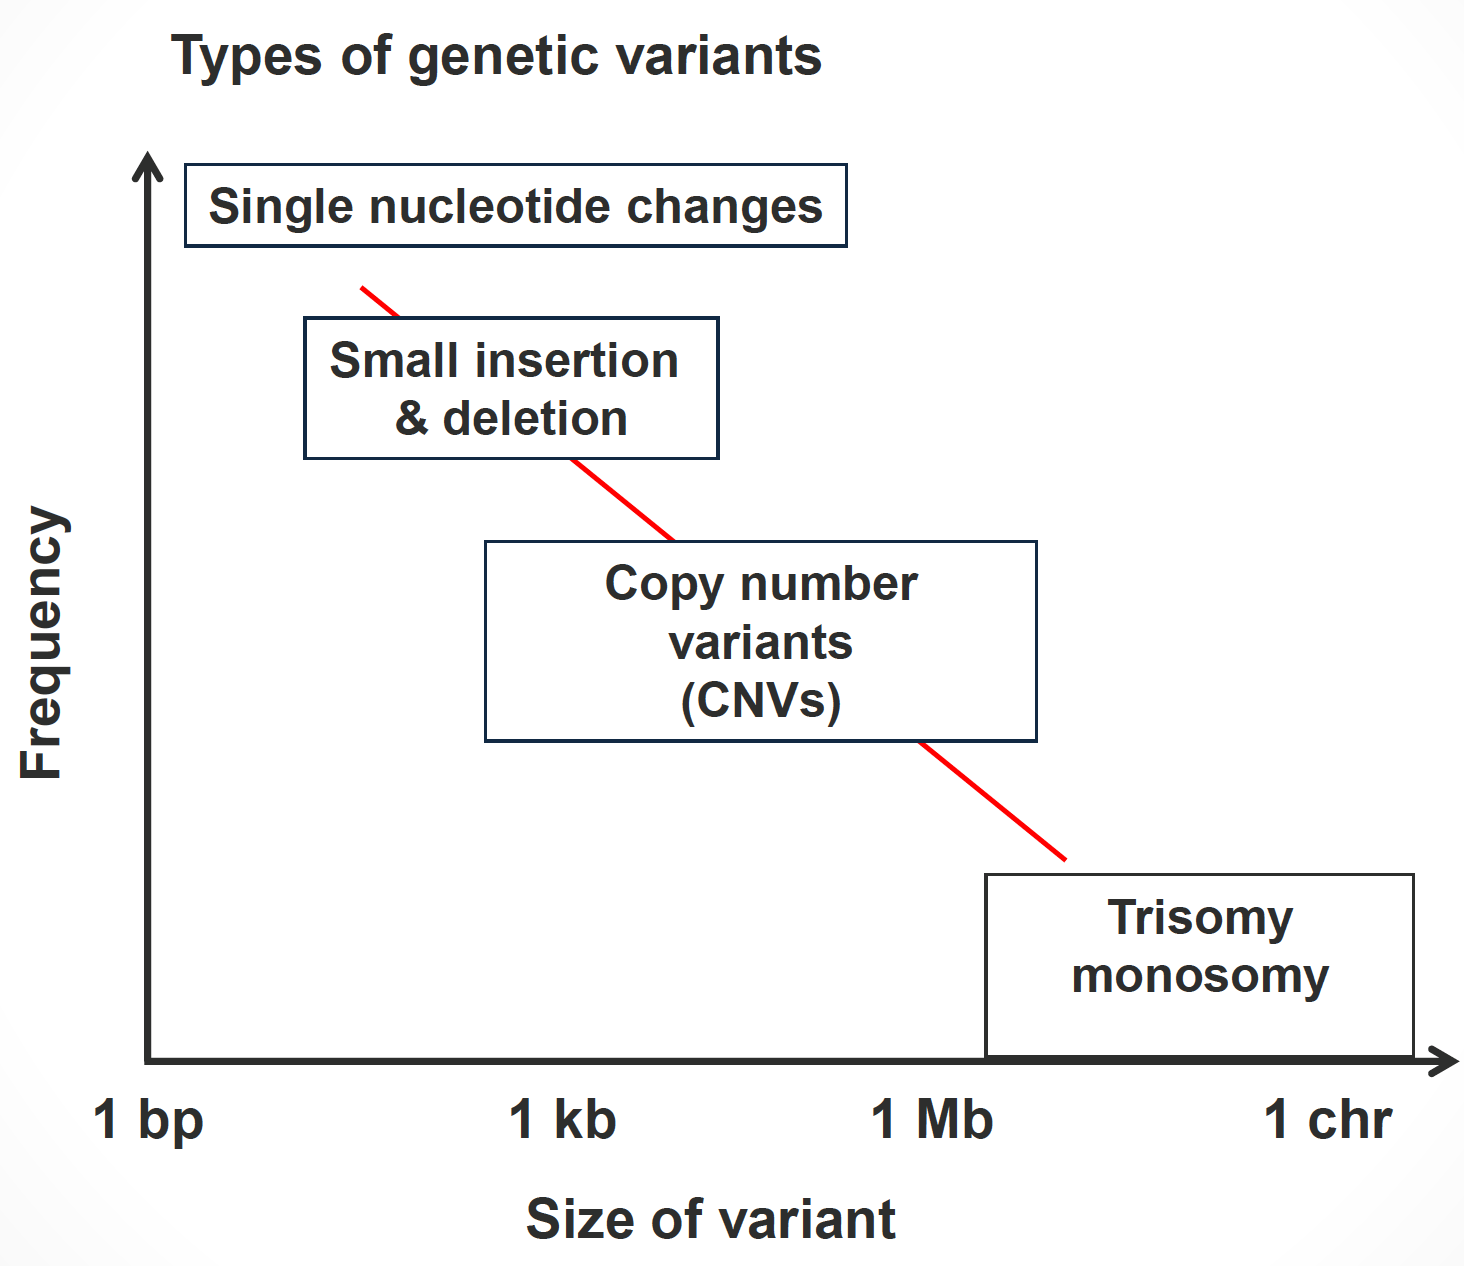
\includegraphics[scale=0.3]{genomicVariation}
\label{geneticVariants}
\end{figure}



\subsection{Single Nucleotide Polymorphism}
Single nucleotide polymorphism, SNP for short, is a substitution at a specific position in the DNA sequence. A substitution can be called a SNP if and only if it is the case for more than 1\% percent of the population. The implications of a SNP can be significant especially if it exists in a coding region of the DNA. A SNP can change the translation of a codon into an amino acid, what is called a non-synonymous mutation, causing a distortion in the structure of the protein. 


\subsection{Structural Variation}
Structural variations (SV) are rearrangements in human genome affecting more than 50 bp that could reach up to several megabases. Structural variations can be categorized according to whether they alter the amount of DNA (copy number variations) or not (balanced rearrangements). 

\subsubsection{Copy Number Variation (CNV)}
Copy number variation, also known as unbalanced rearrangement, is a structural variation that changes the amount of DNA. CNVs are also seperated into two:
\begin{itemize}
  \item Insertions and Deletions: As the name suggests, these are insertions or deletions affecting more than 50 bp.
  \item Segmental Duplications: They are segments in the DNA that are more than 1000 basepair and 90\% or more identical. It can be intra-chromosomal as well as inter-chromosomal. Although segmental duplications account for $\sim$5\% of the genome, they are significant because (1) they often exist in gene-rich chromosomes \cite{bailey2002recent} and (2) they are the most active regions in human genome triggering instabilities and new variations in the chromosome \cite{samonte2002segmental,sudmant2010diversity}.
\end{itemize}
\subsubsection{Balanced Rearrangements}
Balanced rearrangements are structural variations that do not change the amount of DNA. Balanced rearrangements can be categorized into two;

\begin{itemize}
    \item Inversions: They are rearrangements where a segment of the DNA is simply inverted.
    \item Translocations: They are rearrangements where two segments of the DNA exchange their locations. 
\end{itemize}

\subsection{Chromosomal Changes}
Chromosomal changes are variations in the number of chromosome-pairs. They are such major variations that they can be detected by a microscope. It can be categorized into three:

\begin{itemize}
    \item Monosomy: It is a chromosomal change where there is only one copy of a chromosome.
    \item Trisomy: It is a chromosomal change where there is an extra copy of a chromosome.
    \item Uniparental Disomy: It is a chromosomal change where both pairs of chromosome come from the same parent.
\end{itemize}

\section{Our Contribution}
In this thesis, we present ParaCoND to discover paralog specific copy numbers for genes residing in segmental duplications. This remains an open problem until mrCaNaVaR \cite{alkan2009personalized} came out, due to the difficult nature of duplicated regions in genome. However, mrCaNaVaR was not good at differentiating the paralogs. Instead it computes aggregate copy number and assigns it to different copies of genes. Accurate prediction of paralog gene copy number paves the way of finding the main cause of a genetic disease. For example; opsin is a gene family responsible for color vision. It has three copies that regulate color vision according to wavelengths of different colors. Therefore a variation on each paralog could have an effect on viewing colors of different wavelengths.

The main improvement of ParaCoND over mrCaNaVaR is that our method utilizes single nucleotide differences among paralogs which helps us to differentiate paralogs from each other. In addition to that, mrCaNaVaR requires a multiple read mapping sequence alignment file, which is not as widespread as unique read mapping. Our method compute the absolute copy numbers of genes residing in segmental duplications using a unique mapping sequence alignment file. 

The organization of the thesis is as follows: We briefly introduced the problem in Chapter 1. We further explain the problem and present our method in Chapter 2. We show the experimental results in Chapter 3. We conclude the thesis with final remarks in Chapter 4. 